% Search for all the places that say "PUT SOMETHING HERE".

\documentclass[11pt]{article}
\usepackage{amsmath,textcomp,amssymb,graphicx,enumerate,hyperref,enumitem,mathtools,tikz-qtree,listings,chemformula,bm,graphicx,grffile,gensymb,physics,amssymb,datetime,siunitx,multicol,pgfplots}
\graphicspath{{/Users/jonathansun5/Documents/Fall 2017/MCB 166/Homeworks/Final/Screen Shot 2017-12-05 at 10.14.41 PM.png} {/Users/jonathansun5/Documents/Fall 2017/MCB 166/Homeworks/Final/Screen Shot 2017-12-05 at 10.41.28 PM.png} {/Users/jonathansun5/Documents/Fall 2017/MCB 166/Homeworks/Final/Screen Shot 2017-10-10 at 8.07.09 AM.png} {/Users/jonathansun5/Documents/Fall 2017/MCB 166/Homeworks/Final/Screen Shot 2017-12-11 at 3.37.00 AM.png} {/Users/jonathansun5/Documents/Fall 2017/MCB 166/Homeworks/Final/Screen Shot 2017-12-11 at 10.33.06 AM.png} {/Users/jonathansun5/Documents/Fall 2017/MCB 166/Homeworks/Final/Screen Shot 2017-12-11 at 11.04.34 AM.png}}
\pgfplotsset{compat=1.14}
\makeatletter
\newcommand{\leqnos}{\tagsleft@true\let\veqno\@@leqno}
\newcommand{\reqnos}{\tagsleft@false\let\veqno\@@eqno}
\newcolumntype{R}[1]{>{\raggedleft\arraybackslash}p{#1}}
\newcolumntype{L}[1]{>{\raggedright\arraybackslash}p{#1}}
\reqnos
\makeatother

\def\Name{Jonathan Sun}  % Your name
\def\SID{25020651}  % Your student ID number
\def\Homework{Final Exam} % Number of Homework
\def\Session{Fall 2017}


\title{MCB166 --- \Session --- \Homework}
\author{\Name, SID \SID}
\markboth{MCB166 --- \Session --- \Homework --- \Name}{MCB166 --- \Session --- \Homework --- \Name}
\pagestyle{myheadings}
\newdate{date}{11}{12}{2017}
\date{\displaydate{date}}

\def\endproofmark{$\Box$}
\newenvironment{proof}{\par{\bf Proof:}}{\endproofmark\smallskip}

\usepackage[margin=1in]{geometry}



\begin{document}
\maketitle

\newpage
\begin{enumerate}[label=\arabic*.]
\item
\textbf{Membrane potentials in a retinal rod}
\vspace*{1\baselineskip}
\\
Consider a membrane permeable to \ch{Na+}, \ch{K+}, and \ch{Cl-} with relative permeabilities, $P_{\ch{Na}}$, $P_{\ch{K}}$, and $P_{\ch{Cl}}$. Assume the ions all obey the constant-field current voltage curve
\begin{align*}
\text{(1) }I_x = F P_x Z_x v \left([X]_o - [X]_i \text{exp}(v)\right) / (1 - \text{exp}(v)).
\end{align*}
Here $v = eV / kT = V / 25 \text{mV}$, $X$ is the concentration of species $x$ in mM, $F$ is the Faraday constant, and $Z_x$ is the valence of species $x$.
\vspace*{1\baselineskip}
\\
We want to compare current-voltage relations and reversal potentials for two different ion channels. One is the typical imperfectly-selective potassium channel (\ch{K}-ch), for which $\alpha_{\text{K}} = P_{\ch{K}} / P_{\ch{Na}} = 50$. The other is a cation channel (Cat-ch), such as is found in postsynaptic and sensory-receptor membranes, for which $\alpha_{\text{U}} = P_{\ch{K}} / P_{\ch{Na}} = 1$.
\vspace*{1\baselineskip}
\\
For a vertebrate photoreceptor, the internal and external ion concentrations are:
\begin{align*}
[\ch{K}]_o = 5 \text{mM; } [\ch{Na}]_o = 120 \text{mM;} \\
[\ch{K}]_i = 125 \text{mM; } [\ch{Na}]_i = 12 \text{mM.}
\end{align*}
\begin{enumerate}[label=(\alph*)]
\item
Use equation (1) for the \ch{Na+} and \ch{K+} currents to derive the GHK equation for the reversal potential of a channel permeable to both \ch{Na} and \ch{K}. Write the reversal potential formula in terms of the relative permeabilities, $\alpha_{\text{K}}$ and $\alpha_{\text{U}}$ of the two channels.
\vspace*{1\baselineskip}
\\
Using equation (1), I can get the equations for \ch{Na+} and \ch{K+}:
\begin{align*}
I_{\ch{Na}} = F P_{\ch{Na}} Z_{\ch{Na}} v \frac{[\ch{Na}]_o - [\ch{Na}]_i e^v} {1 - e^v}
\end{align*}
\begin{align*}
I_{\ch{K}} = F P_{\ch{K}} Z_{\ch{K}} v \frac{[\ch{K}]_o - [\ch{K}]_i e^v} {1 - e^v}
\end{align*}
Since $Z_x$ is the valence and their valences are $1$:
\begin{align*}
I_{\ch{Na}} = F P_{\ch{Na}} \frac{V} {25 \text{mV}} \frac{[\ch{Na}]_o - [\ch{Na}]_i e^{\frac{V} {25 \text{mV}}}} {1 - e^{\frac{V} {25 \text{mV}}}}
\end{align*}
\begin{align*}
I_{\ch{K}} = F P_{\ch{K}} \frac{V} {25 \text{mV}} \frac{[\ch{K}]_o - [\ch{K}]_i e^{\frac{V} {25 \text{mV}}}} {1 - e^{\frac{V} {25 \text{mV}}}}
\end{align*}
Because $I_{\text{total}} = I_{\ch{Na}} + I_{\ch{K}}$:
\begin{align*}
I_{\text{total}} = I_{\ch{Na}} + I_{\ch{K}} = 0
\end{align*}
\begin{align*}
F P_{\ch{Na}} \frac{V} {25 \text{mV}} \frac{[\ch{Na}]_o - [\ch{Na}]_i e^{\frac{V} {25 \text{mV}}}} {1 - e^{\frac{V} {25 \text{mV}}}} + F P_{\ch{K}} \frac{V} {25 \text{mV}} \frac{[\ch{K}]_o - [\ch{K}]_i e^{\frac{V} {25 \text{mV}}}} {1 - e^{\frac{V} {25 \text{mV}}}} = 0
\end{align*}
\begin{align*}
P_{\ch{Na}} \left([\ch{Na}]_o - [\ch{Na}]_i e^{\frac{V} {25 \text{mV}}}\right) + P_{\ch{K}} \left([\ch{K}]_o - [\ch{K}]_i e^{\frac{V} {25 \text{mV}}}\right) = 0
\end{align*}
\begin{align*}
P_{\ch{Na}} [\ch{Na}]_o - P_{\ch{Na}} [\ch{Na}]_i e^{\frac{V} {25 \text{mV}}} + P_{\ch{K}} [\ch{K}]_o - P_{\ch{K}} [\ch{K}]_i e^{\frac{V} {25 \text{mV}}} = 0
\end{align*}
\begin{align*}
P_{\ch{Na}} [\ch{Na}]_i e^{\frac{V} {25 \text{mV}}} + P_{\ch{K}} [\ch{K}]_i e^{\frac{V} {25 \text{mV}}} = P_{\ch{Na}} [\ch{Na}]_o + P_{\ch{K}} [\ch{K}]_o
\end{align*}
\begin{align*}
e^{\frac{V} {25 \text{mV}}} \left(P_{\ch{Na}} [\ch{Na}]_i  + P_{\ch{K}} [\ch{K}]_i\right) = P_{\ch{Na}} [\ch{Na}]_o + P_{\ch{K}} [\ch{K}]_o
\end{align*}
\begin{align*}
e^{\frac{V} {25 \text{mV}}} = \frac{P_{\ch{Na}} [\ch{Na}]_o + P_{\ch{K}} [\ch{K}]_o} {P_{\ch{Na}} [\ch{Na}]_i  + P_{\ch{K}} [\ch{K}]_i}
\end{align*}
\begin{align*}
\ln{e^{\frac{V} {25 \text{mV}}}} = \ln{\frac{P_{\ch{Na}} [\ch{Na}]_o + P_{\ch{K}} [\ch{K}]_o} {P_{\ch{Na}} [\ch{Na}]_i  + P_{\ch{K}} [\ch{K}]_i}}
\end{align*}
\begin{align*}
\frac{V} {25 \text{mV}} = \ln{\frac{P_{\ch{Na}} [\ch{Na}]_o + P_{\ch{K}} [\ch{K}]_o} {P_{\ch{Na}} [\ch{Na}]_i  + P_{\ch{K}} [\ch{K}]_i}}
\end{align*}
\begin{align*}
V = 25 \text{mV} \ln{\frac{P_{\ch{Na}} [\ch{Na}]_o + P_{\ch{K}} [\ch{K}]_o} {P_{\ch{Na}} [\ch{Na}]_i  + P_{\ch{K}} [\ch{K}]_i}}
\end{align*}
With $\alpha_{\ch{K}} = \frac{P_{\ch{K}}} {P_{\ch{Na}}} = 50$:
\begin{align*}
V_{rev} = 25 \text{mV} \ln{\frac{[\ch{Na}]_o + \alpha_{\ch{K}} [\ch{K}]_o} {[\ch{Na}]_i + \alpha_{\ch{K}} [\ch{K}]_i}} = 25 \text{mV} \ln{\frac{[\ch{Na}]_o + 50 [\ch{K}]_o} {[\ch{Na}]_i + 50 [\ch{K}]_i}}
\end{align*}
With $\alpha_{\ch{U}} = \frac{P_{\ch{K}}} {P_{\ch{Na}}} = 1$:
\begin{align*}
V_{rev} = 25 \text{mV} \ln{\frac{[\ch{Na}]_o + \alpha_{U} [\ch{K}]_o} {[\ch{Na}]_i + \alpha_{U} [\ch{K}]_i}} = 25 \text{mV} \ln{\frac{[\ch{Na}]_o + [\ch{K}]_o} {[\ch{Na}]_i + [\ch{K}]_i}}
\end{align*}



\item
Using the GHK equation calculate the reversal potentials for the two chennels \ch{K}-ch and Cat-ch. Insert these values for the batteries in a parallel equivalent circuit for the vertebrate photoreceptor. Label the batteries $E_O$ and $E_L$. Here the subscript ``O'' denotes the imperfect \ch{K} channel open all the time, and the subscript ``L'' denotes the light-sensitive channel, which for a vertebrate rod closes in the light.
\vspace*{1\baselineskip}
\\
For $E_O$:
\begin{align*}
V_{rev} = 25 \text{mV} \ln{\frac{[\ch{Na}]_o + 50 [\ch{K}]_o} {[\ch{Na}]_i + 50 [\ch{K}]_i}} = 25 \text{mV} \ln{\frac{120 \text{mM} + 50 \times 5 \text{mM}} {12 \text{mM} + 50 \times 125 \text{mM}}} = -70.719 \text{mV}
\end{align*}
For $E_L$:
\begin{align*}
V_{rev} = 25 \text{mV} \ln{\frac{[\ch{Na}]_o + [\ch{K}]_o} {[\ch{Na}]_i + [\ch{K}]_i}} = 25 \text{mV} \ln{\frac{120 \text{mM} + 5 \text{mM}} {12 \text{mM} + 125 \text{mM}}} = -2.292 \text{mV}
\end{align*}



\item
For a retinal rod, the membrane potential in the dark is $V_m = -40 \text{mV}$. In the light, the membrane hyperpolarizes to $-70 \text{mV}$. Using the GHK equation, calculate the relative membrane permeabililities, $\beta = (P_{\ch{Na}} / P_{\ch{K}})$ in the light ($\beta_L$) and in the dark ($\beta_D$). These needn't be the same as the relative permeabilities for the individual channels in part (b).
\begin{align*}
V_m = 25 \text{mV} \ln{\frac{\beta [\ch{Na}]_o + [\ch{K}]_o} {\beta [\ch{Na}]_i + [\ch{K}]_i}}
\end{align*}
\begin{align*}
\frac{V_m} {25 \text{mV}} = \ln{\frac{\beta [\ch{Na}]_o + [\ch{K}]_o} {\beta [\ch{Na}]_i + [\ch{K}]_i}}
\end{align*}
\begin{align*}
e^{\frac{V_m} {25 \text{mV}}} = \frac{\beta [\ch{Na}]_o + [\ch{K}]_o} {\beta [\ch{Na}]_i + [\ch{K}]_i}
\end{align*}
\begin{align*}
\beta [\ch{Na}]_i e^{\frac{V_m} {25 \text{mV}}} + [\ch{K}]_i e^{\frac{V_m} {25 \text{mV}}} = \beta [\ch{Na}]_o + [\ch{K}]_o
\end{align*}
\begin{align*}
\beta [\ch{Na}]_i e^{\frac{V_m} {25 \text{mV}}} - \beta [\ch{Na}]_o = -[\ch{K}]_i e^{\frac{V_m} {25 \text{mV}}} + [\ch{K}]_o
\end{align*}
\begin{align*}
\beta = \frac{-[\ch{K}]_i e^{\frac{V_m} {25 \text{mV}}} + [\ch{K}]_o} {[\ch{Na}]_i e^{\frac{V_m} {25 \text{mV}}} - [\ch{Na}]_o}
\end{align*}
\begin{align*}
\beta = \frac{-125 \text{mM} \times e^{\frac{V_m} {25 \text{mV}}} + 5 \text{mM}} {12 \text{mM} \times e^{\frac{V_m} {25 \text{mV}}} - 120 \text{mM}}
\end{align*}
Since $V_m = -40 \text{mV}$ in the dark:
\begin{align*}
\beta_{D} = \frac{-125 \text{mM} \times e^{\frac{-40 \text{mV}} {25 \text{mV}}} + 5 \text{mM}} {12 \text{mM} \times e^{\frac{-40 \text{mV}} {25 \text{mV}}} - 120 \text{mM}} = 0.172
\end{align*}
Since $V_m = -70 \text{mV}$ in the light:
\begin{align*}
\beta_{L} = \frac{-125 \text{mM} \times e^{\frac{-70 \text{mV}} {25 \text{mV}}} + 5 \text{mM}} {12 \text{mM} \times e^{\frac{-70 \text{mV}} {25 \text{mV}}} - 120 \text{mM}} = 0.022
\end{align*}



\item
Draw an equivalent circuit for a membrane having these two types of channel. Write an equation for the membrane reversal potential as a function of the relative conductance $r = g_L / g_O$. Calculate $r$ in the light, and in the dark.
\begin{center}
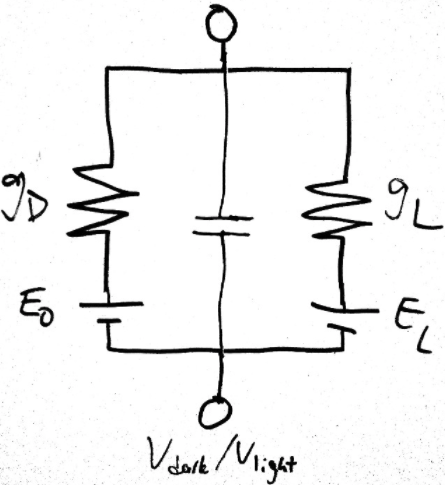
\includegraphics[width=0.5\textwidth]{/Users/jonathansun5/Documents/Fall 2017/MCB 166/Homeworks/Final/Screen Shot 2017-12-11 at 3.37.00 AM.png}
\end{center}
\begin{align*}
I_{\text{total}} = I_O + I_L
\end{align*}
\begin{align*}
I_{\text{total}} = g_O (V - E_O) + g_L (V - E_L)
\end{align*}
Since $r = \frac{g_L} {g_O}$:
\begin{align*}
I_{\text{total}} = 0 = (V - E_O) + r (V - E_L)
\end{align*}
\begin{align*}
r (V - E_L) = -V + E_O
\end{align*}
\begin{align*}
r = \frac{-V + E_O} {V - E_L}
\end{align*}
In the dark:
\begin{align*}
r_D = \frac{-(-40 \text{mV}) + (-70.719 \text{mV})} {-40 \text{mV} - (-2.292 \text{mV})} = 0.815
\end{align*}
In the light:
\begin{align*}
r_L = \frac{-(-70 \text{mV}) + (-70.719 \text{mV})} {-70 \text{mV} - (-2.292 \text{mV})} = 0.011
\end{align*}



\item
Compare the values of $r$ in part (d) with those of ($\beta$) obtained in part (c) and explain any differences.
\vspace*{1\baselineskip}
\\
The values of $r$ are the ratios of conductances while the values of $\beta$ are the ratios of permeabilities. As the permeability ratio increases, the current increases and the conductance also increases.
\end{enumerate}



\newpage
\item
Consider some postsynaptic membrane responses. Use the following ion concentrations:
\begin{align*}
[\ch{K}]_o = 5 \text{mM; } [\ch{Na}]_o = 120 \text{mM; } [\ch{Cl}]_o = 125 \text{mM; } [\ch{Ca}]_o = 5 \text{mM} \\
[\ch{K}]_i = 125 \text{mM; } [\ch{Na}]_i = 12 \text{mM; } [\ch{Cl}]_i = 5 \text{mM; } [\ch{Ca}]_i = 0.005 \text{mM}
\end{align*}
\begin{enumerate}[label=(\alph*)]
\item
Assuming $P_{\ch{K}} : P_{\ch{Na}} : P_{\ch{Cl}} = 1 : 0.02 : 0.1$, use the GHK equation to calculate the membrane resting potential. Ignore the pump, but remember that \ch{Cl} is an anion.
\vspace*{1\baselineskip}
\\
Using the GHK equation:
\begin{align*}
V &= \frac{RT} {F} \ln{\frac{P_{\ch{K}} [\ch{K}]_o + P_{\ch{Na}} [\ch{Na}]_o + P_{\ch{Cl}} [\ch{Cl}]_i} {P_{\ch{K}} [\ch{K}]_i + P_{\ch{Na}} [\ch{Na}]_i + P_{\ch{Cl}} [\ch{Cl}]_o}} \\
 &= 58 \text{mV} \log{\frac{1 \times 5 \text{mM} + 0.02 \times 120 \text{mM} + 0.1 \times 5 \text{mM}} {1 \times 125 \text{mM} + 0.02 \times 12 \text{mM} + 0.1 \times 125 \text{mM}}} \\
 &= 58 \text{mV} \log{\frac{7.9 \text{mM}} {137.74 \text{mM}}} \\
 &= -72.003 \text{mV}
\end{align*}



\item
Assume the threshold depolarization for excitation is $15 \text{mV}$ above the resting potential.
\\
\\
Classify the following postsynaptic channels as being excitatory or inhibitory. Recall that a synapse is excitable if it is capable of depolarizing the membrane \underline{\smash{beyond}} the threshold potential. You have to calculate the reversal potentials for each of these channels.
\begin{center}
\begin{tabular}{ L{3.5em} L{3.25cm} L{4.25cm} L{4.5cm} }
\underline{\smash{Channel}} & \underline{\smash{Selectivity}} & \underline{\smash{Excitatory or Inhibitory?}} & \underline{\smash{Reversal Potential}} \tabularnewline
A. & \ch{Na+} selective & Excitatory. & $E_{\ch{Na}} = \frac{RT} {F} \ln{\frac{[\ch{Na}]_o} {[\ch{Na}]_i}} \newline = 58 \text{mV} \log{\frac{120 \text{mM}} {12 \text{mM}}} \newline = 58 \text{mV}$ \tabularnewline
B. & \ch{K+} selective & Inhibitory. & $E_{\ch{K}} = \frac{RT} {F} \ln{\frac{[\ch{K}]_o} {[\ch{K}]_i}} \newline = 58 \text{mV} \log{\frac{5 \text{mM}} {125 \text{mM}}} \newline = -81.08 \text{mV}$ \tabularnewline
C. & \ch{Cl-} selective & Inhibitory. & $E_{\ch{Cl}} = -\frac{RT} {F} \ln{\frac{[\ch{Cl}]_o} {[\ch{Cl}]_i}} \newline = -58 \text{mV} \log{\frac{125 \text{mM}} {5 \text{mM}}} \newline = -81.08 \text{mV}$ \tabularnewline
D. & Cation selective $\left(P_{\ch{Na}} = P_{\ch{K}}\right)$ & Excitatory. & $E_{P_{\ch{Na}} = P_{\ch{K}}} \newline = \frac{RT} {F} \ln{\frac{[\ch{Na}]_o + [\ch{K}]_o} {[\ch{Na}]_i + [\ch{K}]_i}} \newline = 58 \text{mV} \log{\frac{120 \text{mM} + 5 \text{mM}} {12 \text{mM} + 125 \text{mM}}} \newline = -2.309 \text{mV}$ \tabularnewline
E. & Non-selective pore $\left(P_{\ch{Na}} = P_{\ch{K}} = P_{\ch{Cl}}\right)$ & Excitatory. & $E_{P_{\ch{Na}} = P_{\ch{K}} = P_{\ch{Cl}}} \newline = \frac{RT} {F} \ln{\frac{[\ch{Na}]_o + [\ch{K}]_o + [\ch{Cl}]_i} {[\ch{Na}]_i + [\ch{K}]_i + [\ch{Cl}]_o}} \newline = 58 \text{mV} \log{\frac{120 \text{mM} + 5 \text{mM} + 5 \text{mM}} {12 \text{mM} + 125 \text{mM} + 125 \text{mM}}} \newline = -17.653 \text{mV}$ \tabularnewline
F. & Ligand-gated \ch{Ca} channel & Excitatory. & $E_{\ch{Ca}} = -\frac{RT} {2F} \ln{\frac{[\ch{Ca}]_o} {[\ch{Ca}]_i}} \newline \newline = 29 \text{mV} \log{\frac{5 \text{mM}} {0.005 \text{mM}}} \newline = 87 \text{mV}$ \tabularnewline
\end{tabular}
\end{center}



\item
Some of these channels may not substantially change the membrane potential from rest, but still generate a large conductance change. Are such channels excitatory or inhibitory or neither? Explain. One of these channels may be nominally excitatory, but may not produce a postsynaptic potential change. Which one? There are such channels in some membranes, and their function is related to synaptic plasticity. What might be the function of their very small ionic currents?
\vspace*{1\baselineskip}
\\
Those such channels are inhibitory because they are closer to the threshold value. However, if it is above the resting potential then it is excitatory. The channel that may be nomically excitatory but may not produce a postsynaptic potential change is the Non-selective pore of Channel E. The function of the channels with very small ionic currents is to bring the voltage closer to the threshold and maintain it and therefore make it easier to activate.
\end{enumerate}



\newpage
\item
The figure shows the Hodgkin-Huxley equations and the empirical conductance-gate functions:
\begin{center}
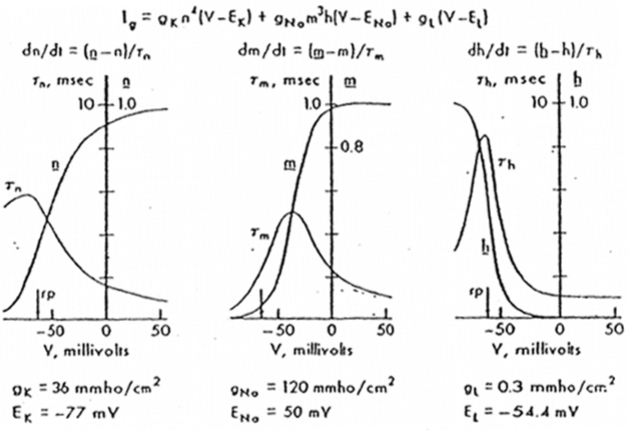
\includegraphics[width=0.75\textwidth]{/Users/jonathansun5/Documents/Fall 2017/MCB 166/Homeworks/Final/Screen Shot 2017-12-05 at 10.14.41 PM.png}
\end{center}
\begin{enumerate}[label=(\alph*)]
\item
Using the data given, plot the steady state current-voltage curve for the \ch{K} channel over the range $-50$ to $+50$ mV from rest.
\vspace*{1\baselineskip}
\\
Since we are working with the \ch{K} channel, $I_{\ch{K}} = \bar{g}_{\ch{K}} n_{\infty}^4 \left(V - E_{\ch{K}}\right)$:
\begin{center}
\begin{tabular}{ l | l | l }
$V$ (mV) & $n_{\infty}$ & $I_{\ch{K}} = \bar{g}_{\ch{K}} n_{\infty}^4 \left(V - E_{\ch{K}}\right)$ \\[0.125cm]
\hline
$-50$ & $0.55$ & $\left(36 \frac{\text{mmho}} {\text{cm}^2}\right) \left(0.55\right)^4 \left(-50 \text{mV} - (-77 \text{mV})\right) = 0.089 \frac{\text{mA}} {\text{cm}^2}$ \\[0.25cm]
$-25$ & $0.8$ & $\left(36 \frac{\text{mmho}} {\text{cm}^2}\right) \left(0.8\right)^4 \left(-25 \text{mV} - (-77 \text{mV})\right) = 0.767 \frac{\text{mA}} {\text{cm}^2}$ \\[0.25cm]
$0$ & $0.9$ & $\left(36 \frac{\text{mmho}} {\text{cm}^2}\right) \left(0.9\right)^4 \left(0 \text{mV} - (-77 \text{mV})\right) = 1.819 \frac{\text{mA}} {\text{cm}^2}$ \\[0.25cm]
$25$ & $0.95$ & $\left(36 \frac{\text{mmho}} {\text{cm}^2}\right) \left(0.95\right)^4 \left(25 \text{mV} - (-77 \text{mV})\right) = 2.991 \frac{\text{mA}} {\text{cm}^2}$ \\[0.25cm]
$50$ & $1$ & $\left(36 \frac{\text{mmho}} {\text{cm}^2}\right) \left(1\right)^4 \left(50 \text{mV} - (-77 \text{mV})\right) = 4.572 \frac{\text{mA}} {\text{cm}^2}$ \\[0.25cm]
\end{tabular}
\end{center}
\begin{center}
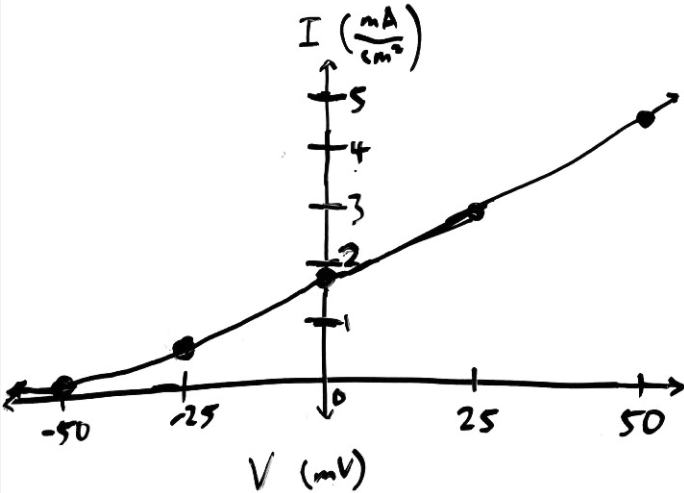
\includegraphics[width=0.5\textwidth]{/Users/jonathansun5/Documents/Fall 2017/MCB 166/Homeworks/Final/Screen Shot 2017-12-11 at 10.33.06 AM.png}
\end{center}



\item
Drugs, such as Yohimbine, can disable the $h$ gate (\ch{Na} inactivation). This will allow \ch{Na} to have a steady-state current-voltage relation. Plot the steady-state I-V curve for the \ch{Na} current in the presence of Yohimbine from $-50$ to $50$ mV.
\vspace*{1\baselineskip}
\\
Since the $h$ gate is disabled, $I_{\ch{Na}} = \bar{g}_{\ch{Na}} m_{\infty}^3 \left(V - E_{\ch{Na}}\right)$:
\begin{center}
\begin{tabular}{ l | l | l }
$V$ (mV) & $n_{\infty}$ & $I_{\ch{Na}} = \bar{g}_{\ch{Na}} m_{\infty}^3 \left(V - E_{\ch{Na}}\right)$ \\[0.125cm]
\hline
$-50$ & $0.2$ & $\left(120 \frac{\text{mmho}} {\text{cm}^2}\right) \left(0.2\right)^3 \left(-50 \text{mV} - (50 \text{mV})\right) = -0.96 \frac{\text{mA}} {\text{cm}^2}$ \\[0.25cm]
$-25$ & $0.8$ & $\left(120 \frac{\text{mmho}} {\text{cm}^2}\right) \left(0.75\right)^3 \left(-25 \text{mV} - (50 \text{mV})\right) = -3.797 \frac{\text{mA}} {\text{cm}^2}$ \\[0.25cm]
$0$ & $0.98$ & $\left(120 \frac{\text{mmho}} {\text{cm}^2}\right) \left(0.98\right)^3 \left(0 \text{mV} - (50 \text{mV})\right) = -5.647 \frac{\text{mA}} {\text{cm}^2}$ \\[0.25cm]
$25$ & $1$ & $\left(120 \frac{\text{mmho}} {\text{cm}^2}\right) \left(1\right)^3 \left(25 \text{mV} - (50 \text{mV})\right) = -3 \frac{\text{mA}} {\text{cm}^2}$ \\[0.25cm]
$50$ & $1$ & $\left(120 \frac{\text{mmho}} {\text{cm}^2}\right) \left(1\right)^3 \left(50 \text{mV} - (50 \text{mV})\right) = 0 \frac{\text{mA}} {\text{cm}^2}$ \\[0.25cm]
\end{tabular}
\end{center}
\begin{center}
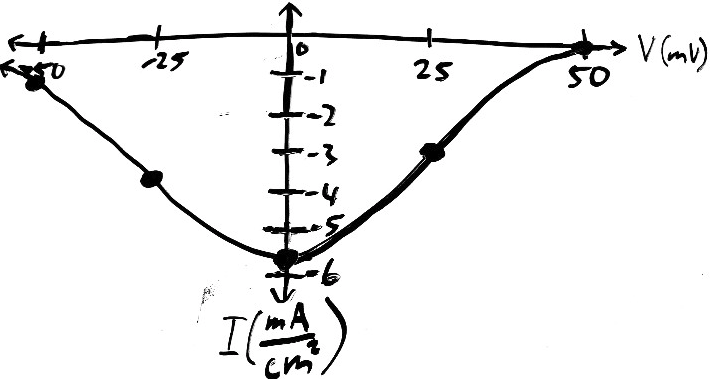
\includegraphics[width=0.5\textwidth]{/Users/jonathansun5/Documents/Fall 2017/MCB 166/Homeworks/Final/Screen Shot 2017-12-11 at 11.04.34 AM.png}
\end{center}



\item
\begin{enumerate}[label=(\roman*)]
\item
Write the expressions for the steady-state current-voltage relations of parts (a) and (b).
\vspace*{1\baselineskip}
\\
For part (a), $I_{\ch{K}} = \bar{g}_{\ch{K}} n_{\infty}^4 \left(V - E_{\ch{K}}\right)$. For part (b), $I_{\ch{Na}} = \bar{g}_{\ch{Na}} m_{\infty}^3 \left(V - E_{\ch{Na}}\right)$ because it is originally $I_{\ch{Na}} = \bar{g}_{\ch{Na}} m_{\infty}^3 h \left(V - E_{\ch{Na}}\right)$ but the $h$ gate is inactivated so we disregard $h$.



\item
Explain how you can separate the two currents by chemical dissection and by ionic substitution.
\vspace*{1\baselineskip}
\\
Blocking \ch{Na} channels by adding TTX or by removing the \ch{Na} outside of the cell will give us $I_{\ch{K}}$. Adding TEA will block \ch{K} channels and give us $I_{\ch{Na}}$.



\item
Explain how you can obtain the instantaneous I-V relations. Use the formulas you just derived in order to aid your explanation, and be precise about the voltage-clamp regimen you would use.
\vspace*{1\baselineskip}
\\
To obtain the instantaneous I-V relations, I chose to find points based off of measurements from $V = -50 \text{mV}$, $V = -25 \text{mV}$, $V = 0 \text{mV}$, $V = 25 \text{mV}$, and $V = 50 \text{mV}$ to calculate the currents at those points. I obtained the $n_{\infty}$ and $m_{\infty}$ values from their respective graphs at their respective voltages and used $I_{\ch{K}} = \bar{g}_{\ch{K}} n_{\infty}^4 \left(V - E_{\ch{K}}\right)$ to calculate the points for the \ch{K} graph and used $I_{\ch{Na}} = \bar{g}_{\ch{Na}} m_{\infty}^3 h \left(V - E_{\ch{Na}}\right)$ to calculate the points for the \ch{Na} graph.



\item
The axon membrane is depolarized by a $140$ mV voltage-clamp step (in the absence of Yohimbine; h is back on again). Calculate the relative contributions of \ch{Na} and \ch{K} to the steady state current (using parameter values from the figure).
\begin{align*}
I_g &= g_{\ch{K}} n_{\infty}^4 \left(V - E_{\ch{K}}\right) + g_{\ch{K}} m_{\infty}^3 h \left(V - E_{\ch{Na}}\right) + g_L \left(V - E_L\right) \\
 &= \left(36 \frac{\text{mmho}} {\text{cm}^2}\right) \left(1\right)^4 \left(140 \text{mV} - (-77 \text{mV})\right) + \left(120 \frac{\text{mmho}} {\text{cm}^2}\right) \left(0\right)^3 \left(140 \text{mV} - (50 \text{mV})\right) \\ &+ \left(0.3 \frac{\text{mmho}} {\text{cm}^2}\right) \left(140 \text{mV} - (-54.4 \text{mV})\right) \\
 &= 7.870 \frac{\text{mA}} {\text{cm}^2}
\end{align*}



\item
Estimate the relative contributions of these two currents at a time $0.5$ msec after the onset of the voltage step (again, h is back on).
\begin{align*}
I = g_{\ch{K}} n_{\infty}^4 \left(V - E_{\ch{K}}\right) + g_{\ch{K}} m_{\infty}^3 \left(V - E_{\ch{Na}}\right) + g_L \left(V - E_L\right)
\end{align*}
\begin{align*}
\frac{dn} {dt} = \frac{n_{\infty} - n} {\tau_n}
\end{align*}
\begin{align*}
\frac{dn} {n_{\infty} - n} = \frac{dt} {\tau_n}
\end{align*}
\begin{align*}
-\ln{(n_{\infty} - n)} = \frac{t} {\tau_n}
\end{align*}
\begin{align*}
n_{\infty} - n = e^{-\frac{t} {\tau_n}}
\end{align*}
\begin{align*}
n = n_{\infty} - e^{-\frac{t} {\tau_n}} = 1 - e^{-\frac{0.5} {0.5}} = 1 - e^{-1} \approx 0.632
\end{align*}
\begin{align*}
m = m_{\infty} - e^{-\frac{t} {\tau_m}} = 1 - e^{-\frac{0.5} {0.01}} \approx 1
\end{align*}
\begin{align*}
h = h_{\infty} - e^{-\frac{t} {\tau_h}} = 0 - e^{-\frac{0.5} {1}} \approx -0.607
\end{align*}
\begin{align*}
I_{\ch{K}} = \bar{g}_{\ch{K}} n_{\infty}^4 \left(V - E_{\ch{K}}\right) = \left(36 \frac{\text{mmho}} {\text{cm}^2}\right) \left(0.632\right)^4 \left(140 \text{mV} - (-77 \text{mV})\right) = 1.246 \frac{\text{mA}} {\text{cm}^2}
\end{align*}
\begin{align*}
I_{\ch{Na}} = \bar{g}_{\ch{Na}} m_{\infty}^3 h \left(V - E_{\ch{Na}}\right) = \left(120 \frac{\text{mmho}} {\text{cm}^2}\right) \left(1\right)^3 \left(-0.607\right) \left(140 \text{mV} - (50 \text{mV})\right) = -6.556 \frac{\text{mA}} {\text{cm}^2}
\end{align*}
\end{enumerate}
\end{enumerate}



\newpage
\item
The figure below shows the equivalent circuit of a postsynaptic cell. The branch with the switch represents the excitatory conductance. Synaptic excitation occurs when the presynaptic neuron fires and all the synaptic ion channels are switched open rapidly. The channels then begin to close randomly, leading to an exponential fall off in synaptically induced conductance.
\begin{center}
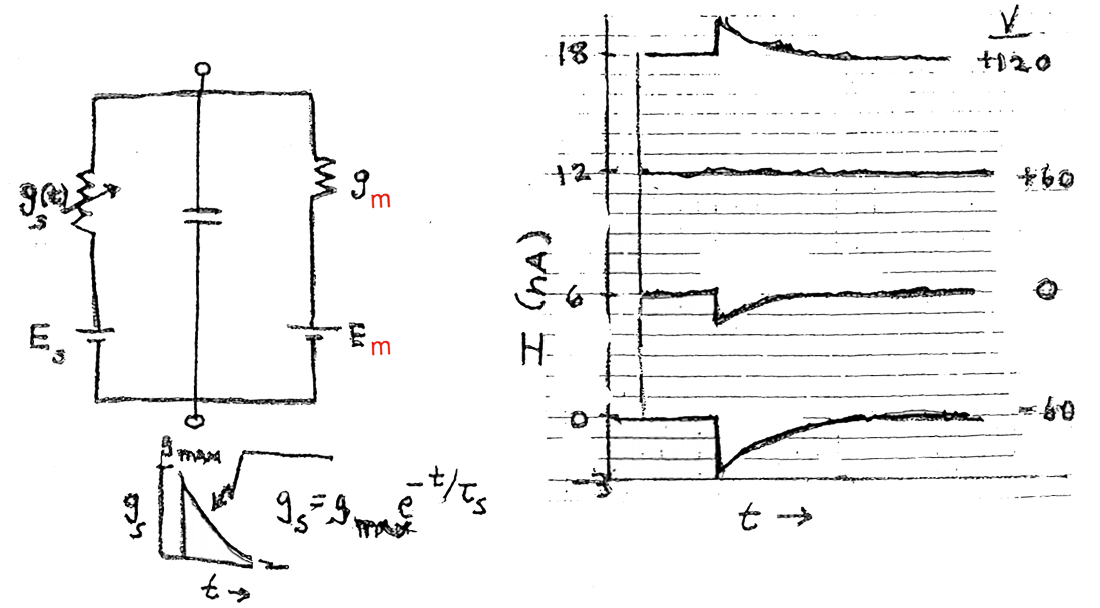
\includegraphics[width=0.75\textwidth]{/Users/jonathansun5/Documents/Fall 2017/MCB 166/Homeworks/Final/Screen Shot 2017-12-05 at 10.41.28 PM.png}
\end{center}
\begin{enumerate}[label=(\alph*)]
\item
The postsynaptic membrane can be voltage-clamped using two microelectrodes. During the clamp pulse the presynaptic nerve is fired, triggering the postsynaptic conductance change. From this voltage clamp data, you can ascertain the current-voltage relations for the resting and synaptic branches. Find the circuit parameters: conductances $g_m$, $g_s$, and reversal potentials $E_m$, $E_s$.
\begin{align*}
g_s = \frac{2 \text{nA} - (-3 \text{nA})} {120 \text{mV} - (-60 \text{mV})} = \frac{5 \text{nA}} {180 \text{mV}} = \frac{1} {36} \text{nS}
\end{align*}
\begin{align*}
g_m = \frac{12 \text{nA} - (0 \text{nA})} {60 \text{mV} - (-60 \text{mV})} = \frac{12 \text{nA}} {120 \text{mV}} = \frac{1} {10} \text{nS}
\end{align*}
\begin{align*}
E_m = E_s = 60 \text{mV}
\end{align*}



\item
Write the differential equation for the time course of the voltage change when the synaptic conductance is abruptly activated at $t = 0$ and subsequently decays exponentially with time constant $\tau_s$. (Hint: write the synaptic conductance as a function, $g_s(t) = g_{\text{max}} \text{exp}(-t / \tau_s)$). Remember that there is no external applied current here, so that $I_{\text{total}} = 0$.
\begin{align*}
I_{\text{total}} = g_m (V - E_m) + g_s (V - E_s) + C \frac{dV} {dt}
\end{align*}
Since $I_{\text{total}} = 0$:
\begin{align*}
0 = g_m (V - E_m) + g_s (V - E_s) + C \frac{dV} {dt}
\end{align*}
\begin{align*}
C \frac{dV} {dt} = -g_m (V - E_m) - g_s (V - E_s)
\end{align*}
\begin{align*}
\frac{dV} {dt} = \frac{-g_m (V - E_m) - g_s (V - E_s)} {C}
\end{align*}
Since $g_s(t) = g_{\text{max}} e^{\frac{-t} {\tau_s}}$:
\begin{align*}
\frac{dV} {dt} = \frac{-g_m (V - E_m) - g_{\text{max}} e^{\frac{-t} {\tau_s}} (V - E_s)} {C}
\end{align*}



\item
Write an expression for the peak depolarization reached during synaptic activation. Calculate the value of peak depolarization from the synaptic equivalent circuit.
\vspace*{1\baselineskip}
\\
Since $\frac{dV} {dt} = 0$ and $I_s = -I_m$:
\begin{align*}
\frac{dV} {dt} = \frac{-g_m (V - E_m) - g_s (V - E_s)} {C} = 0
\end{align*}
\begin{align*}
-g_m (V - E_m) - g_s (V - E_s) = 0
\end{align*}
\begin{align*}
-g_m (V - E_m) = g_s (V - E_s)
\end{align*}
\begin{align*}
-g_m V + g_m E_m = g_s V - g_s E_s
\end{align*}
\begin{align*}
g_m V + g_s V = g_m E_m + g_s E_s
\end{align*}
\begin{align*}
V = \frac{g_m E_m + g_s E_s} {g_m + g_s}
\end{align*}
Plugging in the values we get:
\begin{align*}
V = \frac{\frac{1} {10} \text{nS} \times 60 \text{mV} + \frac{1} {36} \text{nS} \times 60 \text{mV}} {\frac{1} {10} \text{nS} + \frac{1} {36} \text{nS}} = 60 \text{mV}
\end{align*}



\item
If the threshold voltage for initiating an action potential is $V^* = -50 \text{mV}$, is this an excitatory or an inhibitory synapse?
\vspace*{1\baselineskip}
\\
It is an excitatory synapse because $E_s > V^{*}$ ($60 \text{mV} > -50 \text{mV}$).
\end{enumerate}



\newpage
\item
\underline{\smash{\textbf{Gated Ion Channels}}}
\\
\\
Gated ion channels are capable of undergoing rapid conformation changes between non-conducting (closed) and conducting (open) states (C $\rightarrow$ O) due to changes in voltage across the channel. Assume that the energy difference between closed and open states is given by:
\begin{align*}
W_{open} - W_{closed} = -Q_g \left(V - V_0\right)
\end{align*}
\underline{\smash{Where:}}
\\
\textbf{$W_{open} - W_{closed}$:} the difference in energy between open and closed states \\
\textbf{$Q_g$:} gating charge that moves in the membrane \\
\textbf{$Q_g V_0$:} represents some intrinsic, voltage-independent energy differency between two states – described in lecture as the ``conformational'' component of the total energy needed to open the channel.
\begin{enumerate}[label=(\alph*)]
\item
Assuming that the channels in the open and closed states are distributed (at steady state) according to a Boltzmann distribution, derive an expression for the steady-state voltage-dependent conductance of a collection of \textbf{N} gated ion channels of single channel conductance $\gamma$:
\begin{align*}
G_{SS}(V) = N_{\gamma}\left[\frac{1} {1 + exp^{\left(\frac{-Q_g \left(V - V_0\right)} {kT}\right)}}\right]
\end{align*}
\vspace*{1\baselineskip}
\\
Using the Boltzmann Ratio Distribution:
\begin{align*}
\text{Boltzmann Ratio Distribution} = \frac{N_{\text{open}}} {N_{\text{closed}}} = e ^ {- \frac{\Delta W} {k T}}
\end{align*}
Since $N = N_{\text{open}} + N_{\text{closed}}$, we can rearrange it as $N_{\text{closed}} = N - N_{\text{open}}$ and continue:
\begin{align*}
\frac{N_{\text{open}}} {N - N_{\text{open}}} = e ^ {- \frac{\Delta W} {k T}}
\end{align*}
\begin{align*}
N_{\text{open}} = e ^ {- \frac{\Delta W} {k T}} \left(N - N_{\text{open}}\right)
\end{align*}
\begin{align*}
N_{\text{open}} = Ne ^ {- \frac{\Delta W} {k T}} - N_{\text{open}} e ^ {- \frac{\Delta W} {k T}}
\end{align*}
\begin{align*}
N_{\text{open}} + N_{\text{open}} e ^ {- \frac{\Delta W} {k T}} = Ne ^ {- \frac{\Delta W} {k T}}
\end{align*}
\begin{align*}
N_{\text{open}} = \frac{Ne ^ {- \frac{\Delta W} {k T}}} {1 + e ^ {- \frac{\Delta W} {k T}}}
\end{align*}
\begin{align*}
N_{\text{open}} = \frac{N} {e ^ {\frac{\Delta W} {k T}} + 1}
\end{align*}
Since $\Delta W(V) = -Q_g(V - V_0)$:
\begin{align*}
N_{\text{open}} = \frac{N} {e ^ {\frac{-Q_g(V - V_0)} {k T}} + 1}
\end{align*}
\begin{align*}
G_{\text{ss}}(V) = \frac{N_{\gamma}} {1 + e ^ {\frac{-Q_g(V - V_0)} {k T}}}
\end{align*}



\item
\begin{enumerate}[label=(\roman*)]
\item
Sketch the normalized steady state conductance voltage curve (normalized for both the number of channels and the single channel conductance) as a function of voltage (i.e. sketch $\frac{G_{SS}(V)} {N_{\gamma}}$) and indicate on the plot:
\begin{itemize}
\item
the maximum value of $\frac{G_{SS}(V)} {N_{\gamma}}$
\item
the voltage at which half the channels are open
\item
the ``threshold'' region where the steady state conductance is steeply voltage-dependent
\end{itemize}
\begin{center}
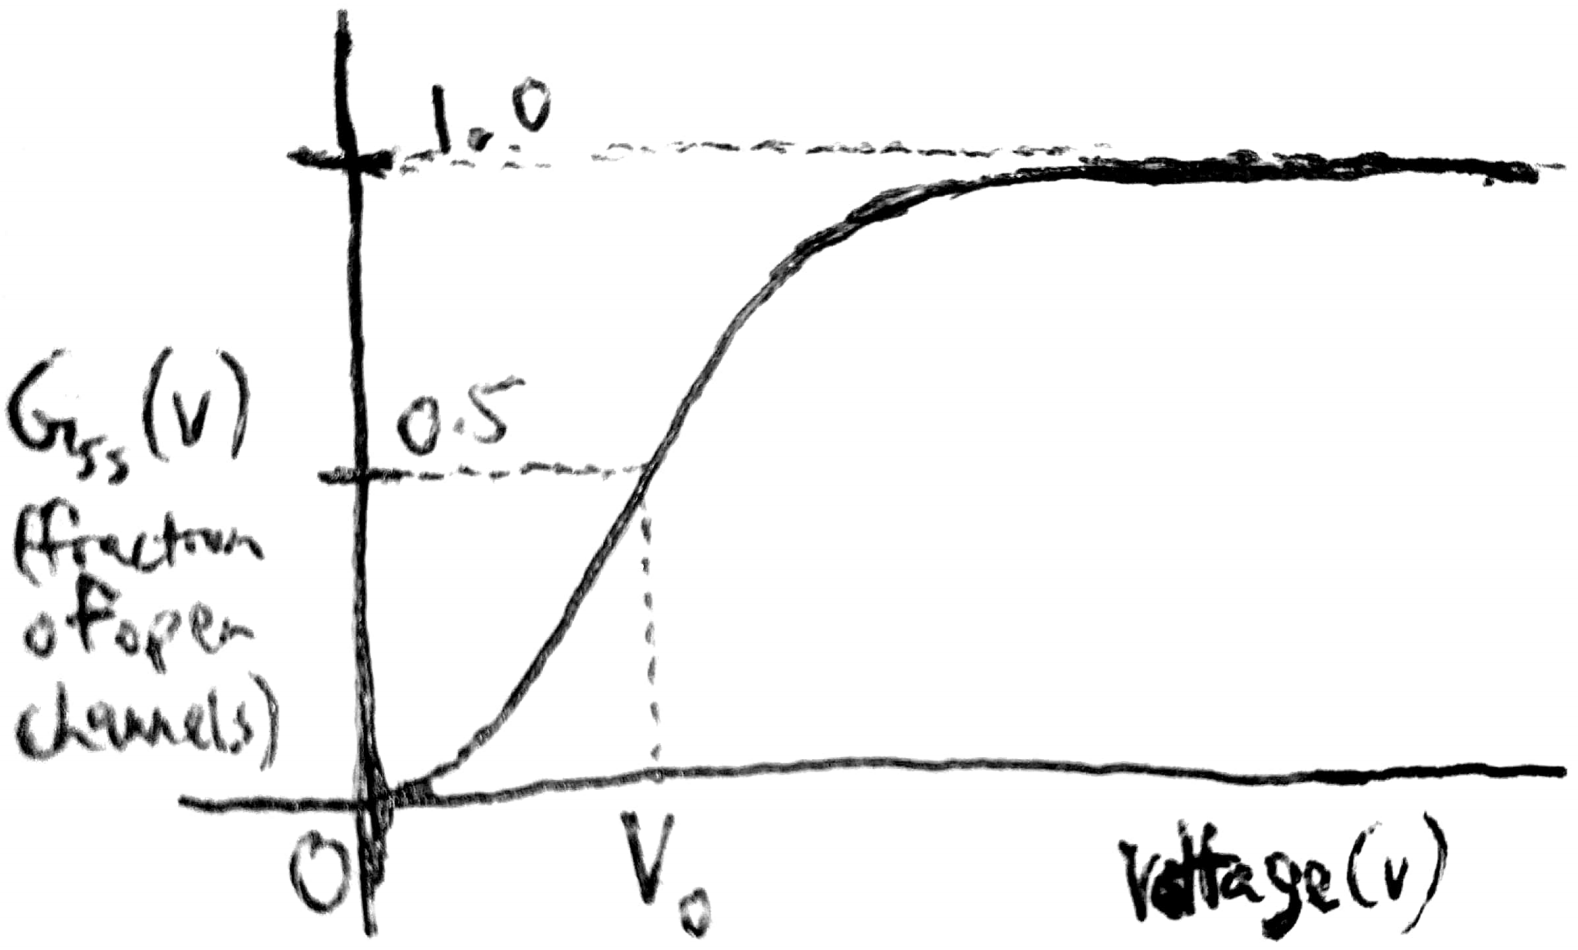
\includegraphics[width=0.75\textwidth]{/Users/jonathansun5/Documents/Fall 2017/MCB 166/Homeworks/Final/Screen Shot 2017-10-10 at 8.07.09 AM.png}
\end{center}
The maximum value of $\frac{G_{\text{ss}}(V)} {N_{\gamma}}$ is $1$ and $\frac{1} {2}$ of the channels are open at $V_0$. The threshold region where the steady state conductance is steeply voltage-dependent is when the slope of the graph is increasing linearly.



\item
How can you determine the gating charge, $Q_g$, from the slope of the steady state conductance versus voltage curve? How will this slope change for different channels with more or less gating charge?
\vspace*{1\baselineskip}
\\
The gating charge, $Q_g$, is proportional to $\delta G$ so that $Q_g$ can be determined from the slope of the graph.



\end{enumerate}
\item
If the channel described in this question is a \ch{Na+} selective channel, then the current-voltage relationship for the \underline{\smash{\textbf{open}}} channel will be:
\begin{align*}
i = \gamma \left(V - V_{\ch{Na}}\right)
\end{align*}
\underline{\smash{Where:}}
\\
$i$: current through a single open channel \\
$\gamma$: single channel conductance (same as in (a)) \\
$V_{\ch{Na}}$: the Nernst potential for sodium
\begin{enumerate}[label=(\roman*)]
\item
Write an expression for $I_{SS}(V)$. Note: the equation above for $i$ above gives the single channel current through an open channel as a function of voltage and $I_{SS}$ is the current at steady state through the population of channels that are open. $i$ is linear with voltage, whereas $I_{SS}$ also depends on how many channels are open at a given voltage. 
\begin{align*}
I_{ss}(V) = G_{SS}(V) (V - E_m) = \frac{N_{\gamma}} {1 + e ^ {\frac{-Q_g(V - V_0)} {k T}}} (V - E_m)
\end{align*}



\item
Sketch the steady state current versus voltage curve for N channels of single channel conductance $\gamma$ for the two different extracellular sodium concentrations below (normalized as above for both the number of channels and the single channel conductance - so plot $\frac{I_{SS}(V)} {N_{\gamma}}$):
\begin{itemize}
\item
$[\ch{Na}]_o = 500 \text{mM}$
\item
$[\ch{Na}]_o = 50 \text{mM}$
\end{itemize}
Assume the following:
$V_0 = 20 \text{mV}$ \\
$\frac{kT} {Q_g} = 5 \text{mV}$ \\
$[\ch{Na}]_i = 50 \text{mM}$
\vspace*{1\baselineskip}
\\
ok.



\item
Indicate any region of negative conductance.
\vspace*{1\baselineskip}
\\
ok.



\end{enumerate}





\item
The slope conductance at any voltage for the $2$ curves plotted in (c) is defined as $\frac{dI(V)} {dV}$. Using the expression found in (c) for $I_{SS}(V)$ what conditions must prevail for there to be a negative conductance region? Would there be a negative conductance for all values of external \ch{Na+} concentration?
\vspace*{1\baselineskip}
\\
ok.
\end{enumerate}



\newpage
\item
\underline{\smash{\textbf{Morphometric Measurements}}}
\\
\textbf{Sholl Analysis}
\\
On the following page you will find tracing of confocal images taken of optic axonal arbors in the brains of \textit{Xenopus} tadpoles. One is a control arbor that only expressed GFP (green fluorescent protein) and the second is a mutant arbor (expressing GFP and a mutant that disrupts $\beta$-catenin adhesive signaling). Each arbor has a set of $9$ concentric circles projected on top of it, centered at the approximate beginning of the arbor. (Ignore the numbers on the branchtips of the arbor.)
\begin{enumerate}[label=(\alph*)]
\item
Please plot a Sholl Analysis for the \# of intersections of the control and mutant arbors with the circles.
\vspace*{1\baselineskip}
\\
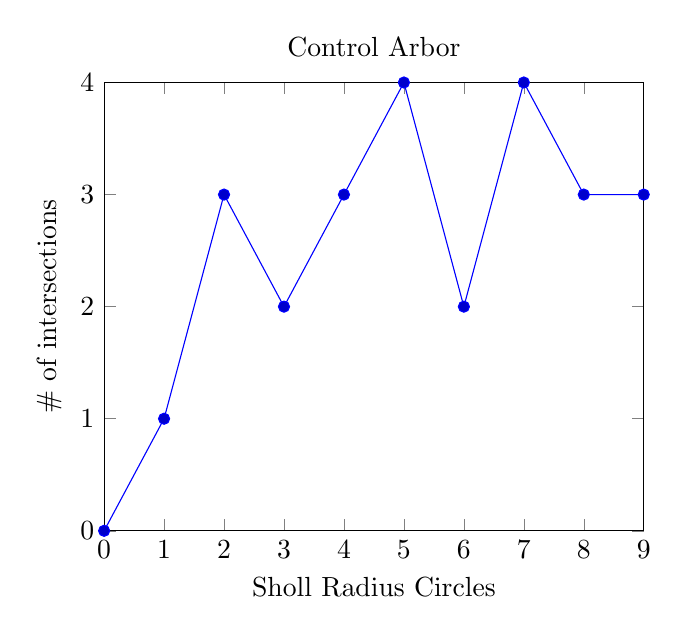
\begin{tikzpicture}
\begin{axis}[
    title={Control Arbor},
    xtick=data,
    xlabel={Sholl Radius Circles},
    ylabel={\# of intersections},
    xmin=0,
    xmax=9,
    ymin=0,
    ymax=4,
    xtick=data]
    \addplot coordinates {
    	(0, 0)
        (1, 1)
        (2, 3)
        (3, 2)
        (4, 3)
        (5, 4)
        (6, 2)
        (7, 4)
        (8, 3)
        (9, 3)
    };
\end{axis}
\end{tikzpicture}
\\
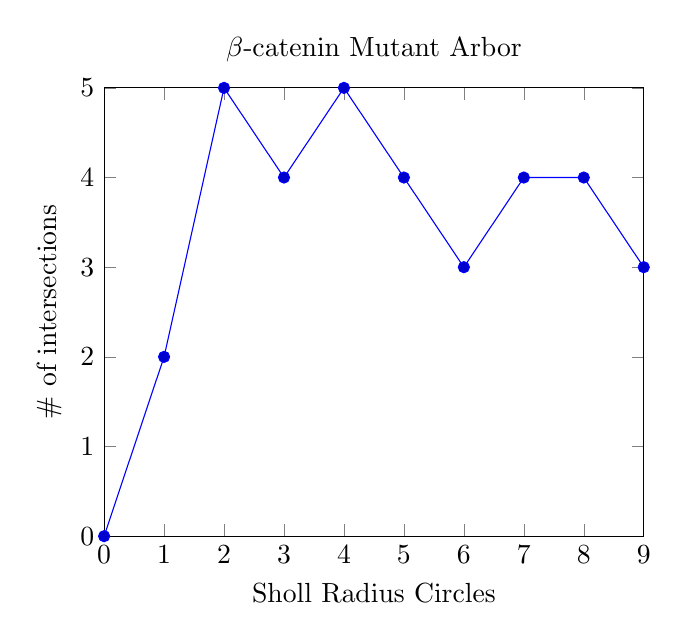
\begin{tikzpicture}
\begin{axis}[
    title={$\beta$-catenin Mutant Arbor},
    xtick=data,
    xlabel={Sholl Radius Circles},
    ylabel={\# of intersections},
    xmin=0,
    xmax=9,
    ymin=0,
    ymax=5,
    xtick=data]
    \addplot coordinates {
    	(0, 0)
        (1, 2)
        (2, 5)
        (3, 4)
        (4, 5)
        (5, 4)
        (6, 3)
        (7, 4)
        (8, 4)
        (9, 3)
    };
\end{axis}
\end{tikzpicture}



\item
Based on your Sholl plots, answer the following question: Do either or both of the arbors show a critical radius (i.e. a circle radius with a maximum number of intersections)? If not, explain why not?
\vspace*{1\baselineskip}
\\
No, none of the arbors show a critical radius. For the Control Arbor, there are two circles, $5$ and $7$, that have $4$ intersections each. For the $\beta$-catenin Mutant Arbor, ther are also two circles, $2$ and $4$, that have $5$ intersections each.



\item
What other differences, if any, do you notice between the Sholl plots of the control and mutant arbors and between the arbors themselves?
\vspace*{1\baselineskip}
\\
I have noticed that at every circle radius, the $\beta$-catenin Mutant Arbor has a higher number of intersections or the same number of intersections compared to the Control Arbor. Also, the axon for the Control Arbor starts from the center of the concentric circles while the axon for the $\beta$-catenin Mutant Arbor starts on the first concentric circle.



\item
How could you improve the Sholl Plots to more realistically show the differences between the arbor branching patterns? What would you expect your Sholl plots to look like if you centered the circles in the middle of the arbors rather than at the beginning of the arbors?
\vspace*{1\baselineskip}
\\
I would put the beginning of the axon for the $\beta$-catenin Mutant Arbor in the center of the concentric circles instead of on the first concentric circle. Doing so would make the $\beta$-catenin Mutant Arbor have more intersections on the higher numbered concentric circles. If I were to center the circles in the middle of the arbors rather than at the beginnnig of the arbors, then the arbors will have more intersections at lower numbered concentric circles than at higher numbered concentric circles.



\item
Can you estimate which arbor has a greater TABL (total arbor branch length)?
\vspace*{1\baselineskip}
\\
The $\beta$-catenin Mutant Arbor has a greater total arbor branch length.
\end{enumerate}
\end{enumerate}
\end{document}
